\chapter{Modifier les styles bibliographiques (2)}

\begin{prealable}
	Nous avons vu que BibLaTeX propose un certain nombres de commandes pour personnaliser rapidement les styles bibliographiques. Toutefois toutes ces commandes ne suffisent pas nécessairement pour des personnalisation avancées. 
	Ainsi la possibilité de choisir l'ordre d'affichage des champs, par exemple, nécessite d'aller plus loin dans la compréhension des styles bibliographiques de de \package{BibLaTeX}.
\end{prealable}



\section{Que se passe-t-il lorsqu'on utilise une commande \commande{cite} ?}

Pour comprendre comment personnaliser l'affichage bibliographique, il est nécessaire de comprendre sommaire ce qui passe lorsqu'on utilise une commande de citation. 

\begin{itemize}
\item Lorsqu'on appelle une commande de citation, du type \verb|PREFXIcite|, cette commande va appeler :
	\begin{itemize}
		\item Des macros bibliographiques, chargées d'afficher l'argument \argument{prenote} ou \argument{postnote}, ou encore de gérer les citations répétées. Les macros bibliographiques sont des types particuliers de commandes, propres au package \package{biblatex}. 
		\item Un driver\footnote{Bien que le terme \enquote{driver} ne soit pas français, nous l'utilisons car il est utilisé dans les commandes internes de BibLaTeX} bibliographique. Un driver correspond à un type d'entrée (@article, @book etc.), et se charge d'afficher les champs de l'entrée dans le bon ordre. Pour ce faire, un driver appelle :
		\begin{itemize}
			\item Des commandes de séparations d'unités bibliographiques, que nous avons vu plus haut.
			\item Des macros bibliographiques. Ces macros bibliographiques appellent elles-même :
			\begin{itemize}
				\item Des commandes d'impression de champs bibliographiques.
				\item Éventuellement d'autres macros bibliographiques.
				\item Des chaînes de langues
			\end{itemize}
		\end{itemize}
		
	\end{itemize}
\end{itemize}

Ceci peut se résumer par le schéma \ref{schema_styles_biblios} (p. \pageref{schema_styles_biblios}). 

\begin{figure}[ht]
\begin{center}
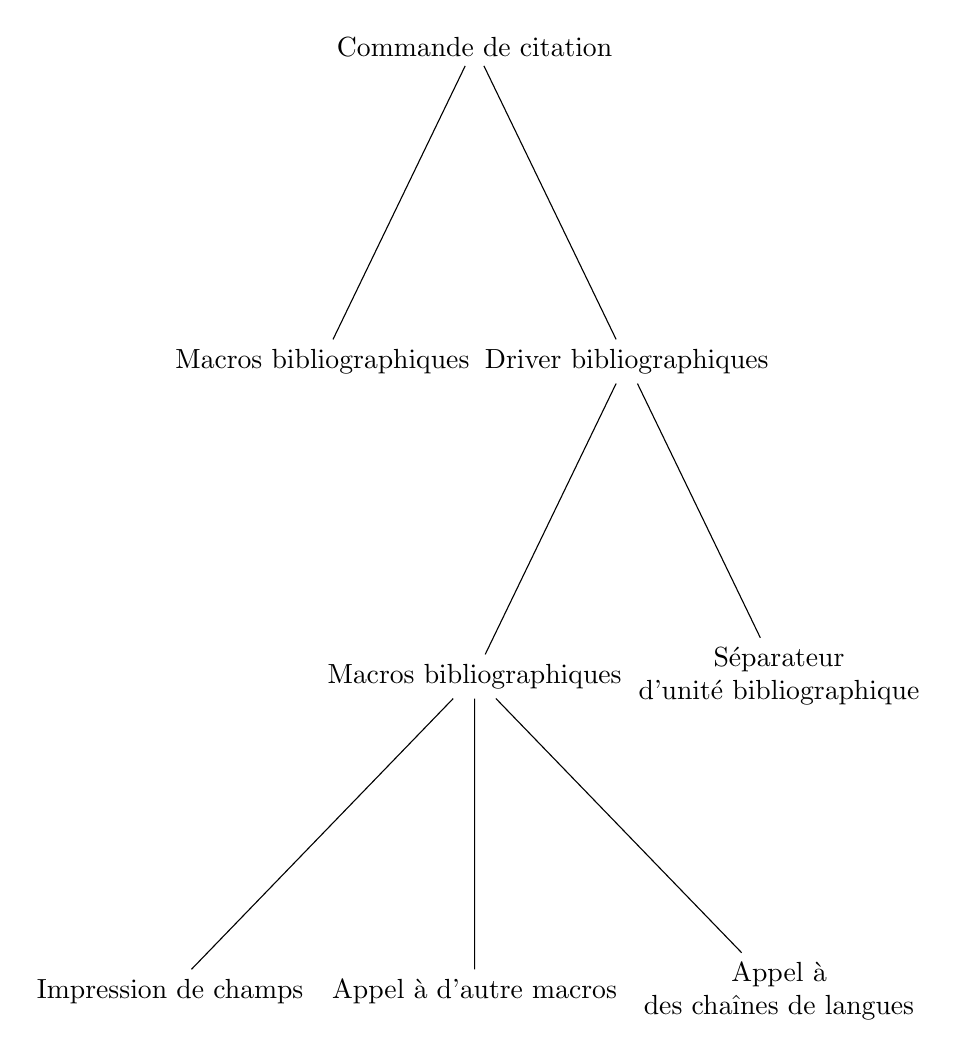
\begin{tikzpicture}[level 1/.style={sibling distance=11em,level distance=4cm},level 2/.style={sibling distance=11em,level distance=4cm},
	every node/.style={align=center}]
	\node {Commande de citation} 
		child { node {Macros bibliographiques}}
		child { node {Driver bibliographiques}
			child { node {Macros bibliographiques}
			 	child {
					node{Impression de champs}
					}
			 	child {
					node{Appel à d'autre macros}
					}
				child {
					node{Appel à \\des chaînes de langues}
					}
				}
			child { node {Séparateur\\ d'unité bibliographique}}
			}	
	;		
\end{tikzpicture}
\end{center}
\caption{Le fonctionnement des styles bibliographiques}\label{schema_styles_biblios}
\end{figure}



\section{Redéfinir une macro bibliographique : l'exemple du champ auteur et éditeur}


L'ensemble de ces éléments sont entièrement redéfinissables. Nous allons prendre un exemple concret de problématique existante.

Prenons l'entrée suivante :

\inputminted{exemples/biblio/fichier/saxer.bib}

Elle s'affiche ainsi, avec l'éditeur commercial avant l'adresse :

\begin{quotation}
\cite{Saxer1980}
\end{quotation}

On pourrait souhaiter avoir l'éditeur après l'adresse, comme ceci : 

\renewbibmacro*{publisher+location+date}{%
  \printlist{publisher}%
  \iflistundef{publisher}
    {\setunit*{\addcomma\space}}
    {\setunit*{\addcolon\space}}%
  \printlist{location}%
  \setunit*{\addcomma\space}%
  \usebibmacro{date}%
  \newunit}

\begin{quotation}
\cite{Saxer1980}
\end{quotation}



La première chose à faire va donc être de repérer quel macro bibliographique modifier. Pour cela, il faut repérer les fichiers de définition des styles bibliographiques. Il en existe plusieurs :

\begin{itemize}
\item Fichier \ext{def} qui définit les styles invariants, quelque soit le style de bibliographie ou de citation choisi.
\item Fichiers \ext{cbx} qui définissent les styles utilisés lors de l'utilisation des commandes \commande{PREFIXcite}.
\item Fichiers \ext{bbx} qui définissent les styles utilisés lors de l'appel à la commande \commande{printbibliography}.
\end{itemize}

Certains fichiers s'appellent mutuellement : ainsi les fichiers \ext{bbx} contiennent les drivers bibliographiques. Ils sont donc appelés par les fichiers \ext{cbx}. Ces appels mutuels entre fichiers permettent de garantir une uniformité entre les styles bibliographiques lors de l'utilisation de \commande{PREFIXcite} et lors de l'utilisation de \commande{printbibliography}.

Nous supposons que nous vous utilisez les styles de la famille \forme{verbose}. En consultant les journaux de compilation et en ouvrant les fichiers standards, vous pouvez aisément remonter au fichier \fichier{standard.bbx}, qui contient les drivers bibliographiques de cette famille.\renvoi{trouverfichier}


Dedans vous pouvez  repérer les lignes suivantes :
\inputminted{exemples/biblio/styles2/driverbook.tex}

Il s'agit d'un driver bibliographique expliquant comment afficher les entrées de type @book. Ce driver fait appel à des macros bibliographiques (les commandes \commande{usebibmacro}). Ces macros sont communes à plusieurs drivers, ce qui permet d'avoir une certaine uniformité de style (par exemple, afin que les noms d'auteurs s'affichent systématiquement de la même façon).

Dans le lot des macros appelées, on constate l'appel à la macro \forme{publisher+location+date}, via la commande

\begin{minted}{latex}
\usebibmacro{publisher+location+date}
\end{minted}

En fouillant un peu le même fichier, on repère l'endroit où la macro est définie :

\inputminted{exemples/biblio/styles2/publisher+location+date.tex}[linenos]

Nous allons commenter succinctement ces lignes, avant d'expliquer comment faire pour inverser l'ordre des deux champs (mais normalement, en lisant nos commentaires, vous devriez comprendre tout de suite). 

\begin{description}
\item[Ligne 1]La commande \commande{newbibmacro*} indique qu'on déclare une nouvelle macro bibliographique, ici \macro{publisher+location+date}. Pour indiquer qu'on redéfinit une macro déjà existant, il faut utiliser la commande \commande{renewbibmacro*}. La définition de la macro se trouve dans les accolades qui suivent.
\item[Ligne2]La commande \commande{printlist} indique qu'on affiche un champ qui pourrait se présenter sous forme de liste, c'est à dire où le mot clef \forme{and} à un sens. Ici il s'agit du champ \champ{location}. \item[Ligne 3]La commande \commande{iflistundef} test la valeur d'un champ qui pourrait être une liste, ici le champ \champ{publisher}. Si ce champ est vide, il exécute le contenu de la première accolade (ligne 4), sinon celui de la seconde (ligne 5).
\item[Ligne 4]Si donc le champ \champ{publisher} est vide, on créé une nouvelle unité bibliographique (\commande{setunit*}) séparée de la précédente par une virgule suivie d'une espace (\commande{addcomma}\commande{space}).
\item[Ligne 5]Si le champ \champ{publisher} n'est pas vide, alors on crée une nouvelle unité bibliographique, séparée de la suivante par deux-points suivi d'une espace (\commande{addcolon}\commande{space}).
\item[Ligne 6]On imprime le champ \champ{publisher}.
\item[Ligne 7]On crée une nouvelle unité bibliographique, séparée de la précédente par une virgule suivie d'un espace. À noter que le champ \champ{publisher} étant vide, on n'aura qu'une seule virgule : nous renvoyons à nos explication antérieure sur les commandes de ponctuation.\renvoi{commandeponctuation}
\item[Ligne 8]On appelle une macro qui se chargera de l'affichage de la date.
\item[Ligne 9]On crée une nouvelle unité bibliographique. Le signe séparateur sera celui définie par la commande \commande{newunitpunct}, vue plus haut.
\end{description}

Pour inverser l'ordre de nos champs, il suffit donc de redéfinir une macro en inversant l'ordre d'impression des champs. Au passage, on ne veut plus des deux points comme séparateurs, ce qui nous permet de supprimer un test conditionnel.


\begin{minted}{latex}
\newbibmacro*{publisher+location+date}{%
  \printlist{publisher}%
    \setunit*{\addcomma\space}%
  \printlist{location}%
  \setunit*{\addcomma\space}%
  \usebibmacro{date}%
  \newunit}
\end{minted}

\newbibmacro*{publisher+location+date}{%
  \printlist{location}%
  \iflistundef{publisher}
    {\setunit*{\addcomma\space}}
    {\setunit*{\addcolon\space}}%
  \printlist{publisher}%
  \setunit*{\addcomma\space}%
  \usebibmacro{date}%
  \newunit}
	% Remettre les champs dans le bon ordre.


Prêtez bien attention aux \% de fin de lignes : les oublier signifie risquer d'avoir des espaces indésirables dans ses références bibliographiques.


\begin{anedocte}

Il  existe d'autres commandes que \commande{printfield} pour imprimer des champs : \commande{printname} pour imprimer un champ contenant des noms de personne, et \commande{printfield} pour imprime un champ ne nécessitant pas de mise en forme particulière.

Pour mieux comprendre quand utiliser l'une ou l'autre de ces commandes, le mieux est de regarder les fichiers standards.

\end{anedocte}
\begin{anedocte}
Si vous utilisez le champ \champ{address} à la place du champ \champ{location}, sachez que le premier est considéré comme un alias du second : autrement dit utiliser \champ{address} revient à utiliser \champ{location}.

On peut déclarer des nouveaux alias de champ via la commande 

\begin{minted}{latex}
\DeclareFieldAlias{alias}{original}
\end{minted}

Mais normalement vous ne devriez pas avoir à utiliser cette commande.
\end{anedocte}

\section{Autres exemples : des véritables \emph{op. cit.}}

Un des éléments gênants des styles bibliographiques standards de la famille verbose est leur manière de gérer les abréviations universitaires de type \emph{op. cit.}. En effet, les styles indiquent les \emph{op. cit.} après avoir affiché l'auteur et le titre. Par exemple :

\begin{quotation}
\cite{Saxer1980}

…

\cite{Saxer1980}
\end{quotation}

Si nous n'avons qu'une seule entrée dont Victor Saxer est l'auteur, cela est assez inutile. On pourrait avoir une version abrégée sous la forme :

% Changeons %
\renewbibmacro*{cite:title}{%
  \printtext[bibhyperlink]{%
   \ifsingletitle{}{\printfield[citetitle]{labeltitle}}%
    \setunit{\nametitledelim}%
    \bibstring[\mkibid]{opcit}}}
% Changeons

\begin{quotation}
\cite{Saxer1980}
\end{quotation}

% Rétablissons
\newbibmacro*{cite:title}{%
  \printtext[bibhyperlink]{%
    \printfield[citetitle]{labeltitle}%
    \setunit{\nametitledelim}%
    \bibstring[\mkibid]{opcit}}}
% Rétablissons

Pour ce faire, nous allons modifier les styles de \emph{BibLaTeX}, en utilisant la commande \commande{ifsingletitle{oui}{non}}. Cette commande vérifie si une entrée est la seule attribuée à son auteur, et renvoie \argument{oui} si c'est le cas, \argument{non} sinon. 

Pour la faire fonctionner, il faut utiliser Biber\renvoi{biber}, et passer l'option \option{singletitle=true} au chargement de \package{biblatex}.

\begin{minted}{latex}
\usepackage[singletitle=true,...]{biblatex}
\end{minted}

Une fois ceci fait, il est nécessaire de savoir où appliquer cette commande. Commençons par fouiller le fichier \ext{cbx}, puisqu'il s'agit d'un style pour une commande \commande{PREFIXcite}. Recherchons l'expression \forme{opcit} qui correspond à la chaîne de langue qui renvoie \forme{op. cit.} (voir chapitre précédent).\renvoi{opcit}.

On repère rapidement qu'elle se trouve dans une macro \macro{cite:title}.

\begin{english}%en attendant que ce bug soit résolu
\inputminted{exemples/biblio/styles2/citetitle.tex}
\end{english}
Procédons à l'analyse :

\begin{description}
\item[Ligne 1]le nom de la macro est \macro{cite:title}.
\item[Ligne 2]la commande \commande{printtexte} sert à deux chose : à mettre directement un texte en s'assurant que BibLaTeX gère la ponctuation ou bien à assembler plusieurs champs dans un seul bloc typographique. Ici, nous avons affaire au second usage. L'argument \argument{bibhyperlink} signifie que \package{BibLaTeX} va s'occuper de mettre un lien hypertexte à l'intérieur du document PDF.
\item[Ligne 3]la commande \commande{printfield} imprime un champ. Ici le pseudo-champ \champ{labeltitle} : celui-ci renvoie la valeur du champ \champ{shortitle} s'il est définie, sinon celle de \champ{title}.\renvoi{shortfields}. Il l'affiche selon le format \argument{citetitle}\footcite[On pourrait si on voulait définir une autre manière d'afficher ce champ grâce à la commande \commande{DeclareFieldFormat}.Voir]{biblatex_formating}.
\item[Ligne 4]nouvelle unité bibliographique, dont le séparateur est défini par la commande \commande{nametitledelim}.
\item[Ligne 5]la commande \commande{bibstring} sert à appeler une chaîne de langue, ici \verb|opcit|. Le premier argument \argument{\commande{mkibid}} sert à indiquer que la chaîne de langue est passée à la commande \commande{mibid} avant d'être affichée.
\end{description}

La ligne qui nous intéresse est donc la ligne 3 : il faudrait conditionner l'affichage du champ titre : si il n'y a qu'une seule œuvre pour l'auteur courant, on peut ne pas l'afficher. Il suffit de redéclarer la macro, en insérant le test conditionnel :

\begin{english}%en attendant que ce bug soit résolu
\inputminted{exemples/biblio/styles2/singletitle.tex}
\end{english}


